% 本章节是介绍实验流程
\section{实验流程}
本文是依据Github上的很多年以前的项目——BusyBear \cite{BusyBear} 来实现的,但是该项目已经有四年没有更新了,在实验过程中,本人发现说明文档中很多步骤以及脚本内容已经不适用了,由于软件的更新迭代还出现很多新问题,比方说当时采用Linux Kernel v4.4,当时Linux主分支不支持RISC-V,但是本文采用现在主流的Linux Kernel版本 Linux Kernel v5.*,该版本的Linux主分支已经支持了RISC-V架构了;还有就是Qemu在4.*的时候需要自己编译 OpenSBI ,但是在Qemu 5.*以后就内嵌 OpenSBI,一些流程也有所改变,但是清楚Linux启动流程就可以了,详细参考《从按下电源开始的一场接力赛》\cite{从按下电源开始的一场接力赛}。

\subsection{前期准备}
本实验环境是在Intel的 x86 平台,实验运行系统是Gentoo linux \cite{Gentoo_AMD64_Handbook},系统具体信息如图\ref{fig:gentoo} 所示。


\begin{figure}[htbp]
  \centering %居中显示
  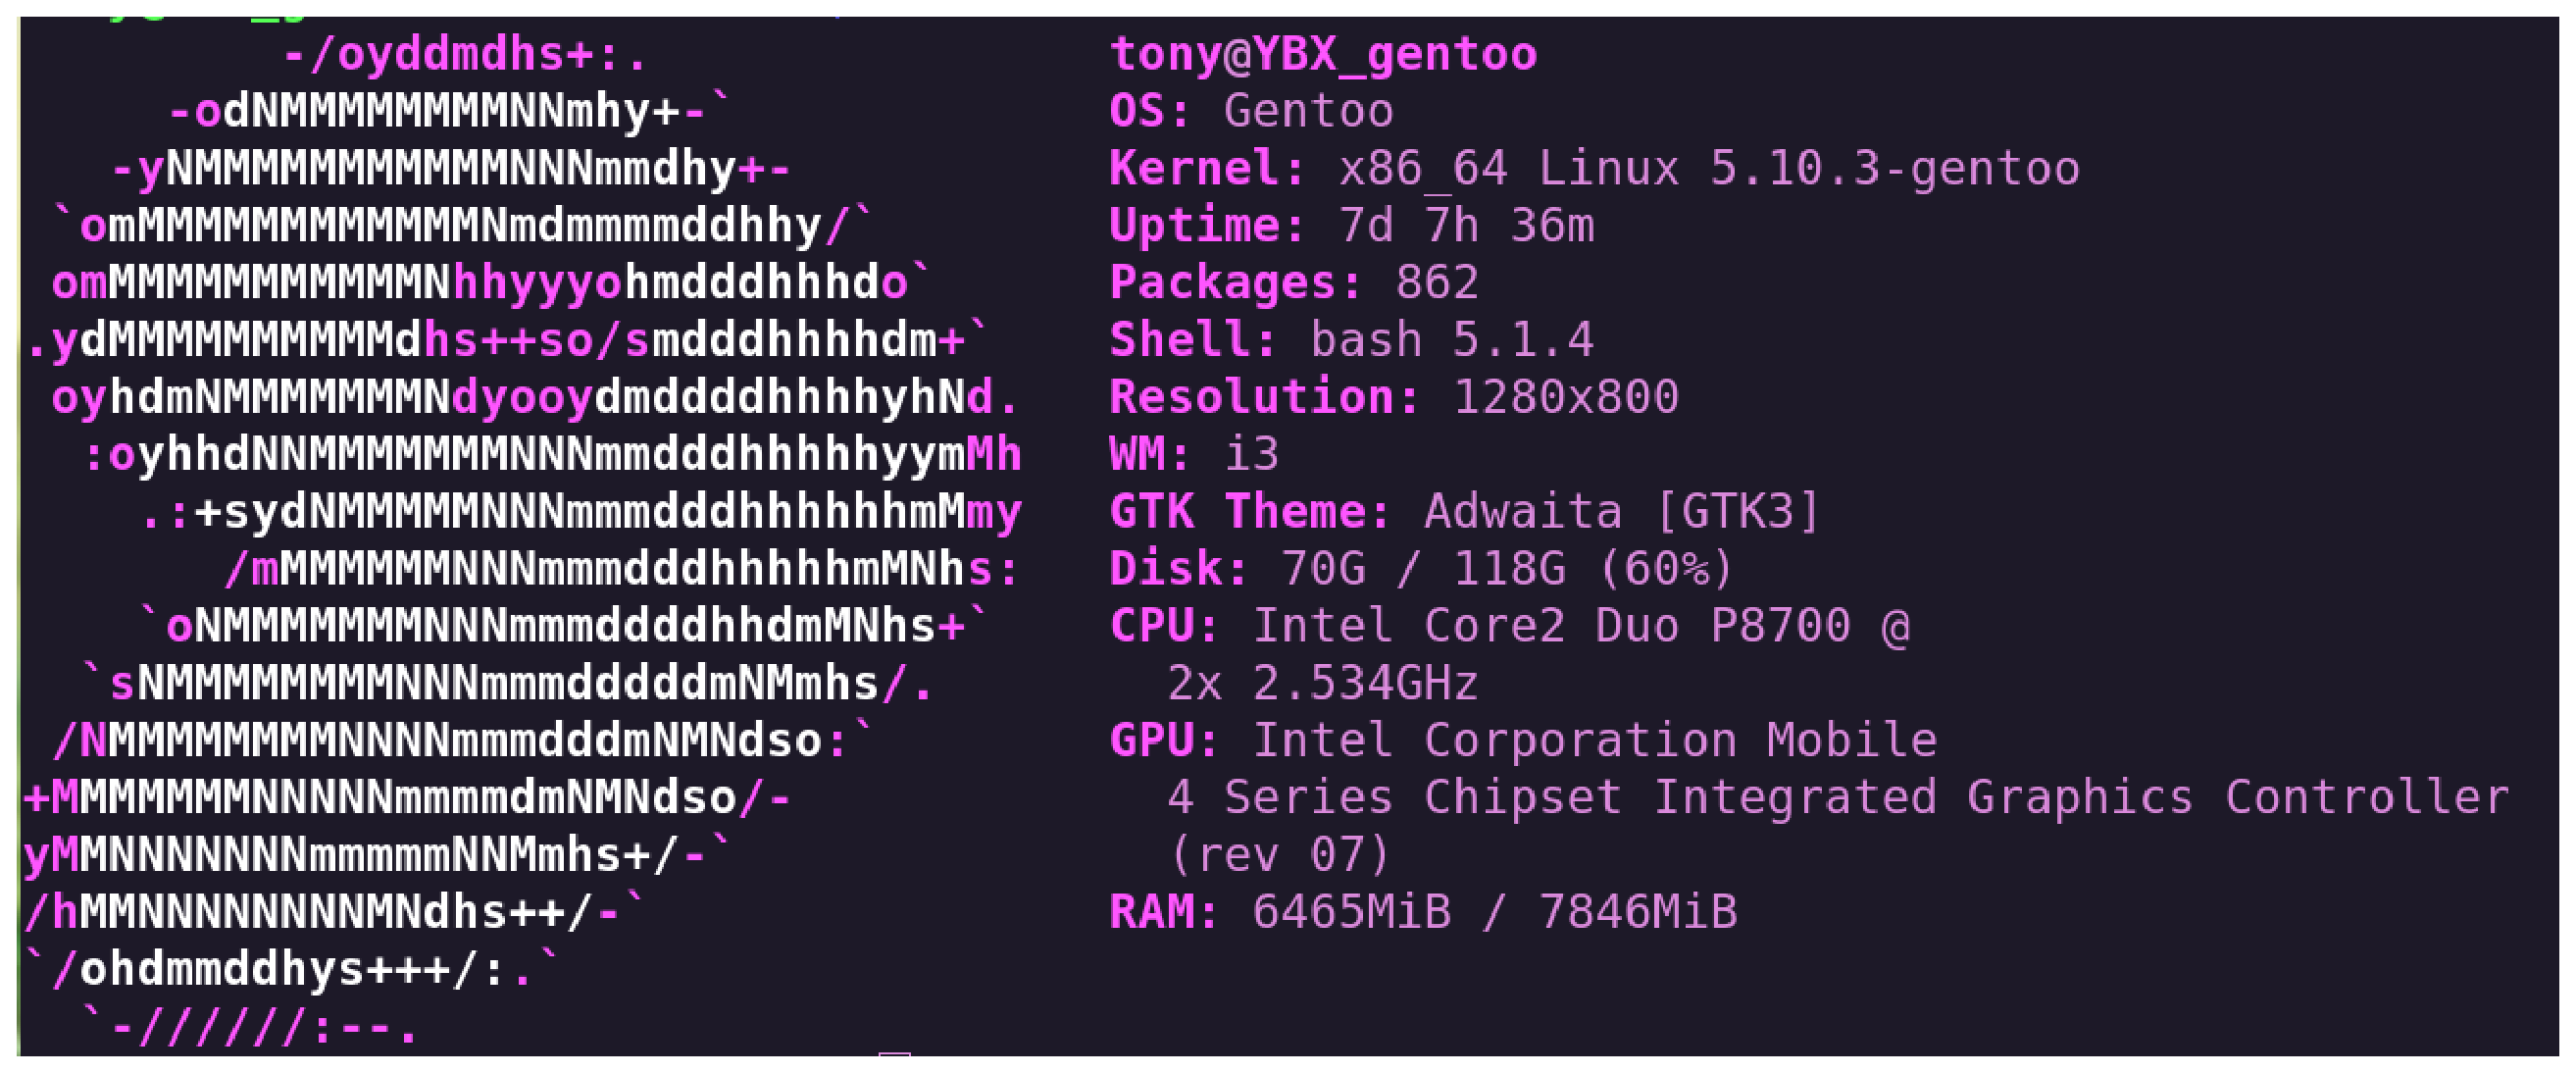
\includegraphics[width=0.8 \textwidth]{figs/Process/gentoo_Logo.eps}
  \caption{实验操作系统}
  \label{fig:gentoo} %设置图形引用名称
\end{figure}

\subsubsection{交叉工具链的准备}
本文我使用的是GNU提供的交叉工具链,实验前需要安装并配置好实验所需的工具链,并根据仓库的 README.md 文档,在x86平台交叉编译出 RISC-V 所需的工具链, 并进行安装与配置  \cite{riscv-binutils-gdb} \cite{riscv-dejagnu} \cite{riscv-gcc} \cite{riscv-glibc} \cite{riscv-newlib} \cite{riscv-pk} ,本实验所需的各种GNU工具链软件信息如图\ref{fig:info}。

其中,这些仓库比较多一个一个下载比较浪费时间,而且加起来也很大,所以后来发现在执行的时候可以递归下载 riscv-gnu-toolchain \cite{riscv-gnu-toolchain} ,可以一次将全部所需的工具链下载完成,最后在使用 Autotool 进行 configure,并根据自身机器进行配置,详细内容可见附录B。


\begin{figure}[htbp]
  \centering %居中显示
  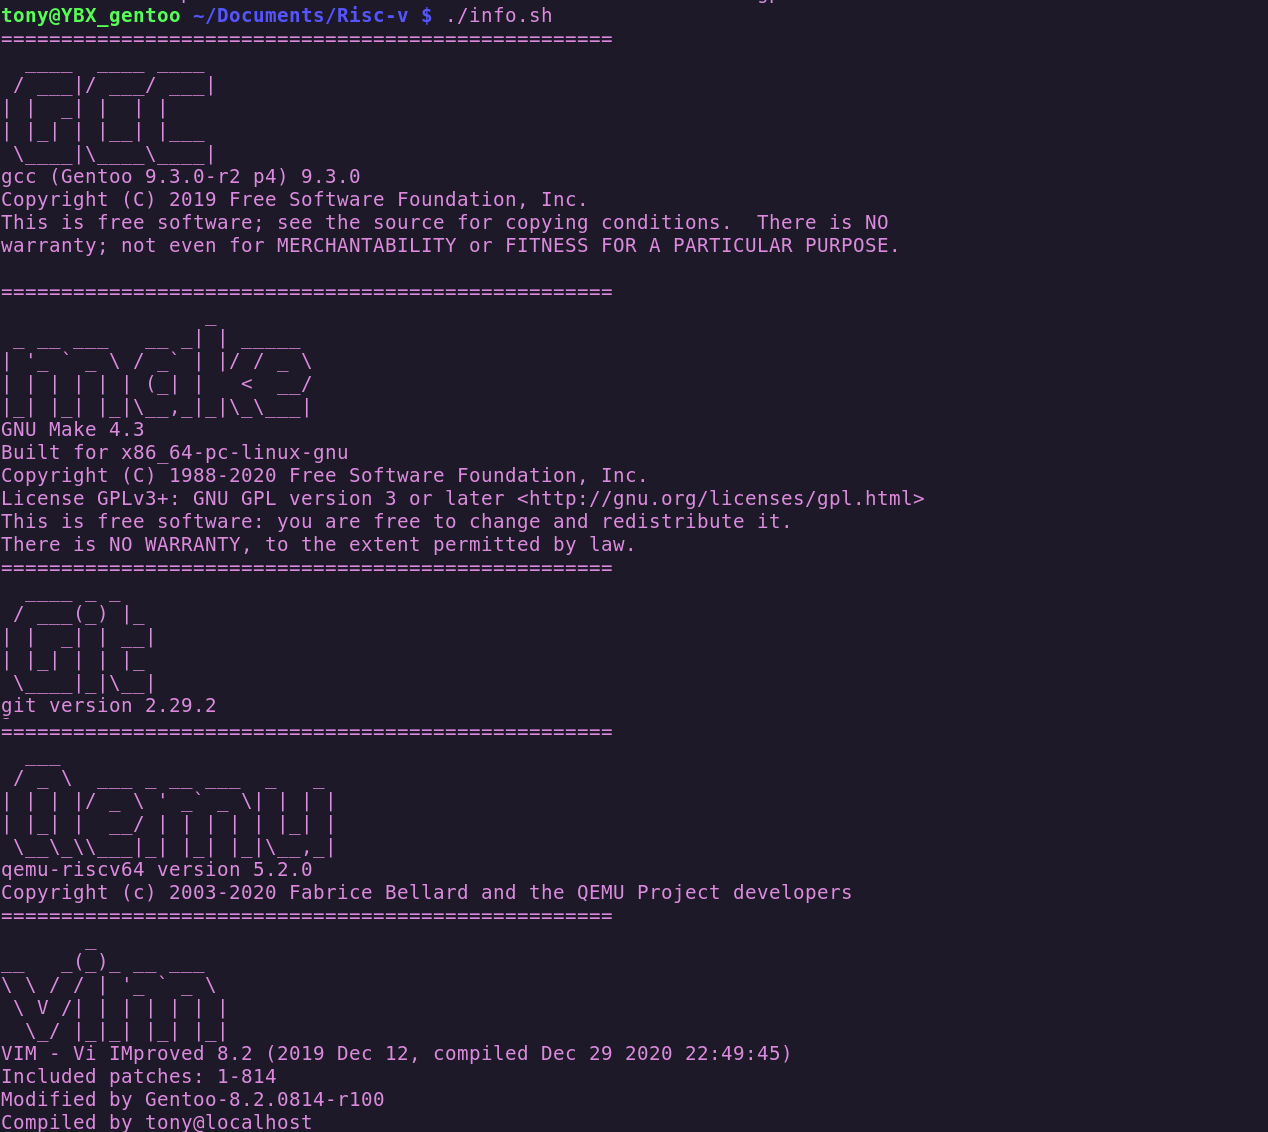
\includegraphics[width=1.0 \textwidth]{figs/Process/info.png}
  \caption{实验所需软件信息}
  \label{fig:info} %设置图形引用名称
\end{figure}

\subsection{Qemu \& KVM搭建}
因为使用的系统环境是 Gentoo Linux ,所以根据 Gentoo 官方的 Wiki 手册中 Qemu 部分来按照步骤完成即可 \cite{GentooQemu} , 主要修改系统中的 USE 来支持RISC-V \cite{KVM安装与配置} ,详细内容可见已经录制好的视频《第一次安装配置Gentoo》\cite{第一次安装配置Gentoo}中 Qemu \& KVM 部分。
% 
\subsection{移植过程介绍}
Linux在 v5.0 以后,既然内核已经可以支持RISC-V,这样只需要在使用 make menuconfig 配置内核的时候加上支持RISC-V的参数,并在make的时候加上选项 ARCH=riscv ,并指定需要的交叉编译器参数即可, 当然编译不是一次就能成功的, 可能已经编译很长时间最后还是失败了, 但是可以根据日志来进行修改配置文件, 最后其他设置就具体情况具体分析即可。

\subsection{制作 BootLoader——BBL(Berkeley Boot Loader)}
这里是根据 riscv-pk \cite{riscv-pk} 中 README.md 的步骤完成实现的。

需要注意的是在编译的时候需要指定risc-v linux Kernel 的最原始未压缩的内核文件—— vmlinux , 完成编译 BootLoader, 具体实现脚本可见附录B。

\subsection{创建根文件系统}
busybon使用了 riscv-qemu 的 virtio-net 与 virtio-block。首先需要使用 qemu-img 生成一块磁盘,用于分区,并存放文件系统。

在busybear的说明文档中有提到可以使用 busybox  来制作文件系统,参考busybox的手册 \cite{busybox} 可以完成其安装配置,并让其完美的运行在Qemu上。

对于文件系统格式化,采用通用的ext4格式,挂载到临时文件夹,并创建根目录所需的一切结构文件夹,结束后要将临时文件夹删除。

\subsection{配置SSH服务}
考虑目前的系统比较简单不完善,所以考虑使用SSH来进行访问与操作。

在给系统实现 SSH 服务时,这里使用dropbear 来实现提供对简单的risc-v 操作系统的SSH服务,其实我想实现SSH操作并且可以外部访问,根据 Dropbear的官方文档\cite{Dropbear} 实现安装与运行操作。

\subsection{最终效果}
最终启动结果如图\ref{fig:success}所示,可以支持SSH访问,如图\ref{fig:ssh_transparent}所示,并且可以执行程序如图\ref{fig:run_truth}所示。
\begin{figure}[htbp]
  \centering %居中显示
  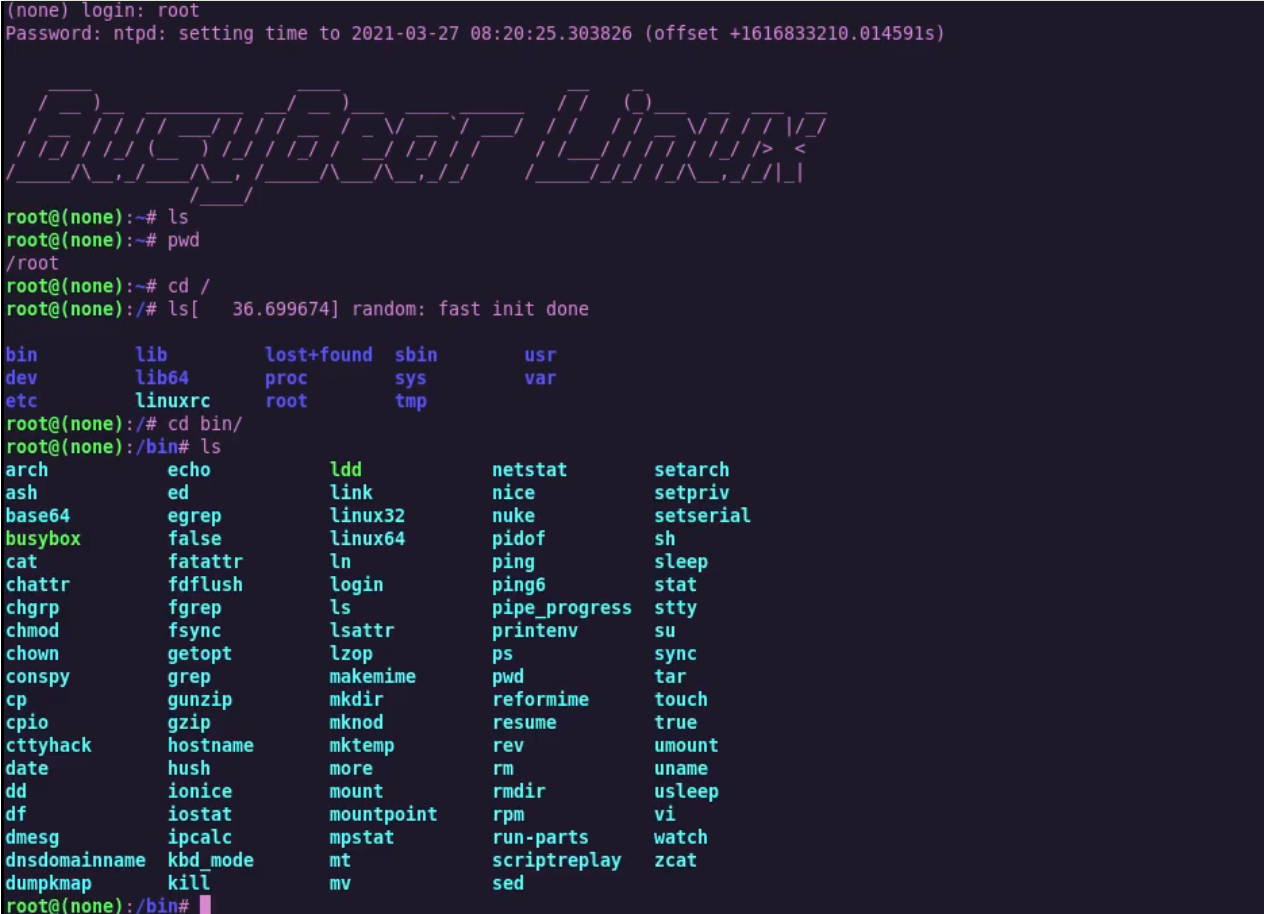
\includegraphics[width=0.9 \textwidth]{figs/Process/success.png}
  \caption{运行成功}
  \label{fig:success} %设置图形引用名称
\end{figure}

\begin{figure}[htbp]
  \centering %居中显示
  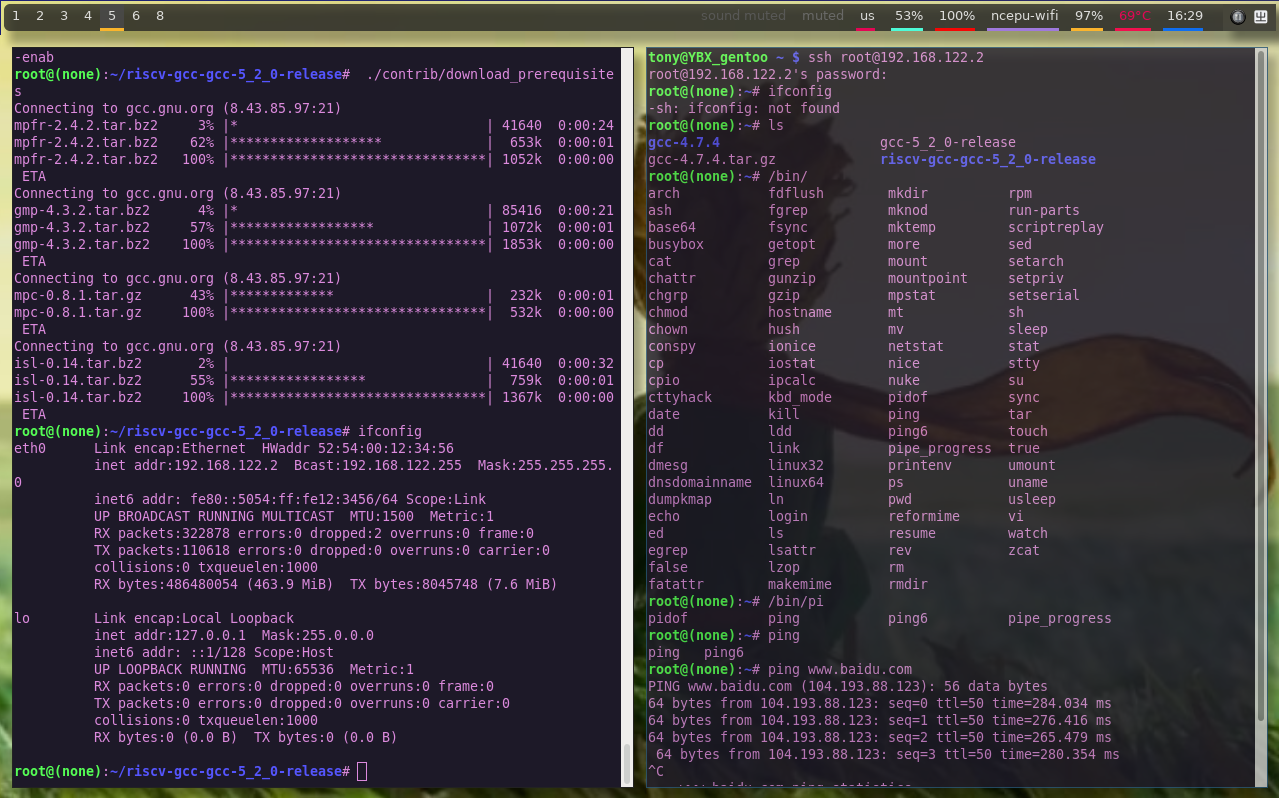
\includegraphics[width=1.0 \textwidth]{figs/Process/ssh_transparent.png}
  \caption{支持SSH网络连接}
  \label{fig:ssh_transparent} %设置图形引用名称
\end{figure}

为了表明自己实验成功是 RISC-V 的, 实现编译好一个 RISC-V 的程序, 来验证该操作系统能否正常的使用, ./truth.riscv 是实现编译好的一个演示程序, 运行结果如图\ref{fig:run_truth}所示,可以正常运行成功。

\begin{figure}[htbp]
  \centering %居中显示
  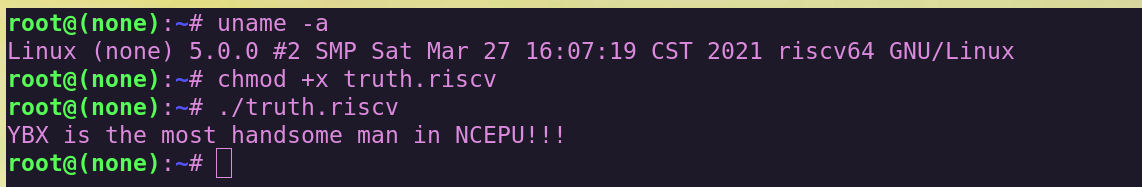
\includegraphics[width=0.9 \textwidth]{figs/Process/run_truth.png}
  \caption{运行程序}
  \label{fig:run_truth} %设置图形引用名称
\end{figure}








